\section{HDAC6 Structure and Function}

One such host protein with the potential to be a drug target is histone deacetylase 6 (HDAC6), along with the molecular motors myosin 10 and dynein, and their respective cytoskeletal filaments \cite{banerjee2014influenza}.

Histone deacetylases are a class of enzymes that remove acetyl groups from chromatin and other acetylated proteins. Currently 18 HDAC proteins are known, which are classified into 4 classes. HDAC6 belongs to the IIb class, which is primarily localized in the cytoplasm \cite{hai2016histone}.

Among other histone deacetylases, HDAC6 is the only one to carry tandem catalytic domains CD1 and CD2 (Figure \ref{figure:HDAC6Domains}). The dynein motor binding (DMB) domain is located between them. HDAC6 also has a ubiquitin-binding domain ZnF ("zinc-finger") which senses polyubiquitinated misfolded protein cargo \cite{hai2016histone}. HDAC6-ZnF selectively binds \cite{zhang2008mice} to ubiquitin chains with unanchored C-terminal diglycine \cite{ouyang2012protein}.

\begin{center}
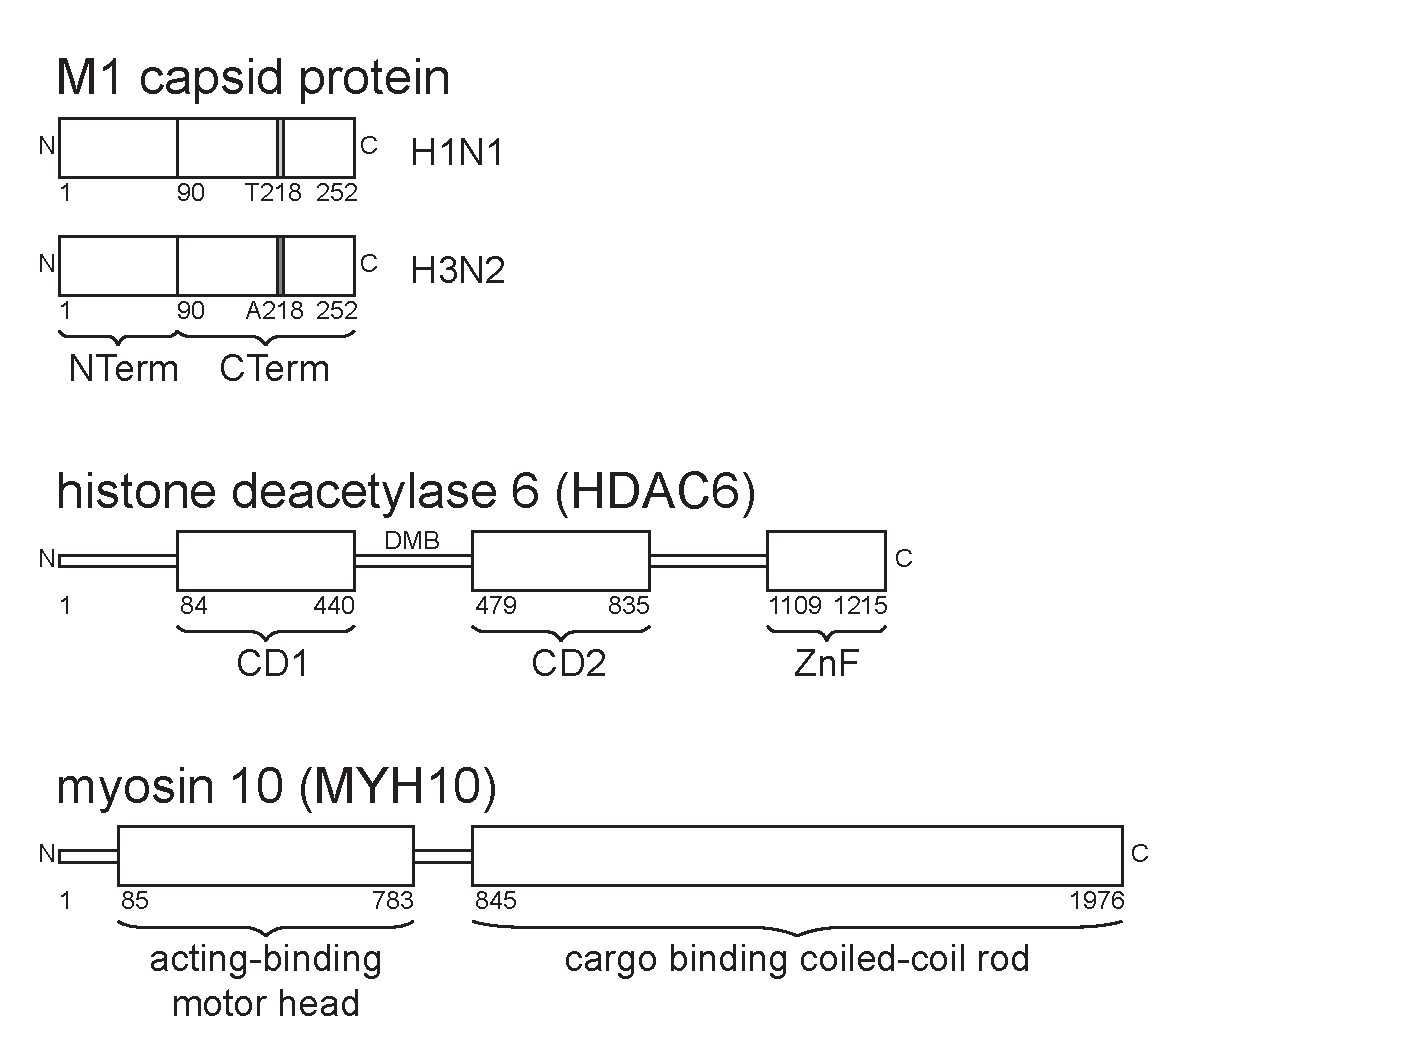
\includegraphics[width=1\textwidth, trim={0cm 6cm 8cm 8.8cm}, clip]{D_chapters/0_introduction/protein_domains.pdf}
\captionof{figure}{HDAC6 domain organization}
\label{figure:HDAC6Domains}
\end{center}

HDAC6 deacetylates tubulin \cite{zhang2003hdac, zhang2008mice} (polymer making up the microtubules), and heat shock protein 90 (Hsp90) \cite{kovacs2005hdac6} (a chaperone protein which assists protein folding and degradation). HDAC6 senses ubiquitinated protein aggregates and triggers their clearance \cite{boyault2007hdac6}. HCAC6 also assists in stress granule formation and cellular oxidative stress recovery \cite{kwon2007deacetylase}.

During influenza infection, HDAC6 (specifically, HDAC6-ZnF) and other components of the aggresome processing machinery - molecular motors myosin 10 and dynein - were essential for efficient uncoating. Involvement of molecular motors suggested that influenza uncoating is achieved through physical forces generated by microtubule- and actin-associated motors \cite{banerjee2014influenza}.

